% 定理1
\begin{theorem}
線形無順序木パターンに対する無矛盾性問題${\cal LUTP}$-${\cal CP}$はNP完全である.
\end{theorem}

\begin{proof}
線形無順序木パターンに対する無矛盾性問題がクラスNPに属すことは自明である.
NP完全であることが知られている充足可能性問題(3-SAT)から${\cal LUTP}$-${\cal CP}$への多項式時間帰着を示す.
$x_{1},\ldots,x_{n}$を$n$ $(n\geq 0)$個の論理変数とし,$x_{1},\ldots,x_{n}$の3つのリテラルからなる節を$C_{1},\ldots,C_{m}$ $(m\geq 0)$とする.
$F=C_{1}\vee\cdots\vee C_{m}$を3-CNFの論理式とする.
任意の$i$ $(1\leq i\leq n)$と$k$ $(1\leq k\leq m)$に対して,$C_{k}$はリテラル$x_i$と$\bar{x_i}$を両方とも含むことはないとしても一般性を失わない.
$F$が充足可能であるとき,そのときに限り,${\cal LUTP}$-${\cal CP}$の問題における条件を満たす線形無順序木パターン$t\in {\cal LUTP}_{\Sigma,\Lambda,X}$が存在するように$S_{+}$と$S_{-}$を構成する.
頂点ラベル,辺ラベルの集合をそれぞれ$\Sigma=\{\varepsilon\}$, $\Lambda=\{0,1,2,\textrm{a},\textrm{b}\}$とする.ここで,$\varepsilon$は空語を表す.
$T$を図\ref{fig:sample-tree}に定める最大深さ$n+1$の無順序木とする.
\begin{enumerate}
\item[(1)] 論理変数$x_{i}$ ($1\leq i\leq n$)に対する無順序木の正例$T_{i}^{(+)}$と負例$T_{i}^{(-)}$ $(1\leq i\leq n)$を次のように構成する:
$T$の深さ$i+1$ $(1\leq i\leq n)$の同じ親を持つ深さ$i+2$の3つの葉のうち,$0$を親への辺の辺ラベルとする葉を削除して得られる無順序木を$T_{i}^{(+)}$ ($1\leq i\leq n$)とする.また,$T$の深さ$i+1$ $(1\leq i\leq n)$の同じ親を持つ深さ$i+2$の3つの葉のうち,$1$または$2$を親への辺の辺ラベルとする葉の1つを削除して,他方の辺ラベルを$0$に変更して得られる無順序木を$T_{i}^{(-)}$ ($1\leq i\leq n$)とする(図\ref{fig:sample-tree}).
$T_{i}^{(+)}$の深さ$i+1$における葉のうち,親への辺の辺ラベル$1$は$x_{i}$の値が$true$であることを,親への辺の辺ラベル$2$は$x_{i}$の値が$false$をあることを表す.
線形無順序木パターン$t$で,$T_{i}^{(+)}\in L(t)$かつ$T_{i}^{(-)}\not\in L(t)$となるものが存在するならば,深さ$i+2$の葉に繋がる辺の辺ラベルによって,$L(t)$に属する無順序木か否かが判断されることに注意する.
なぜなら,$T_{i}^{(+)}$と$T_{i}^{(-)}$の違いは深さ$i+2$の葉に繋がる辺の辺ラベルだけであるからである.
さらに,$T_{i}^{(-)}$の深さ$i+1$の葉の親への辺の辺ラベルが$0$であることから,線形無順序木パターン$t$の深さ$i+1$の葉の親への辺には,辺ラベル$1$または$2$を持つものが存在しなければならない.
\item[(2)] 節$C_{k}$ ($1\leq k\leq m$)に対する無順序木を次のように構成する:
節$C_k$ $(1\leq k\leq m)$が論理変数$x_p,x_q,x_r$ $(1\leq p < q < r \leq n)$のリテラルを含むとき,$T$の深さ$p+1,q+1,r+1$の葉を次のように変更して,負例$T_{n+k}^{(-)}$ $(1\leq k\leq m)$を作成する(図\ref{fig:clause-tree}): $C_k$が含む論理変数$x_p$に対して,$T$の深さ$p+1$の同じ親を持つ3つの葉のうち,$0$を親への辺の辺ラベルとする葉を削除して,$x_p$が正のリテラルのとき,残りの2つの葉の親への辺の辺ラベルを両方とも$2$に,$x_p$が負のリテラルのとき,残りの2つの葉の親への辺の辺ラベルを両方とも$2$にする.$x_q$と$x_r$のリテラルに対しても,$T$の深さ$q+1$と$r+1$の葉に対して同様の操作を行う.このようにして構成した無順序木$T_{n+k}^{(-)}$ $(1\leq k\leq m)$は,$C_{k}$に含まれるリテラルが同時に$false$にならないことを表す.
\end{enumerate}
$S_{+}=\{T_1^{(+)},T_2^{(+)},\ldots,T_n^{(+)}\}\subseteq {\cal UT}_{\Sigma,\Lambda}$,$S_{-}=\{T_1^{(-)},T_2^{(-)},\ldots,T_{n}^{(-)}\}\cup\{T_{n+1}^{(-)},\ldots,T_{n+m}^{(-)}\}\subseteq {\cal UT}_{\Sigma,\Lambda}$とする.図\ref{fig:example_npc}に例をあげる.

\medskip

% 図3.1
\begin{figure}[tb]
  \centering
  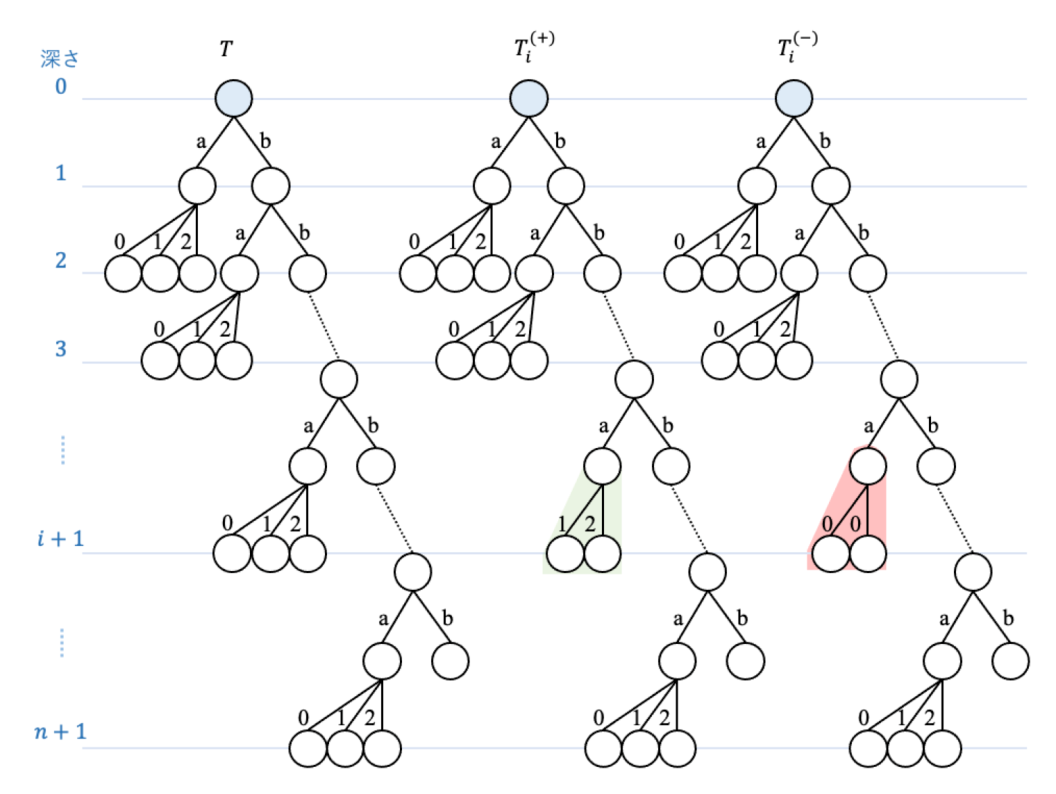
\includegraphics[scale=0.5]{fig/sample-tree.eps}
  \caption{正例と負例の元となる無順序木$T$と正例の無順序木$T_{i}^{(+)}$,負例の無順序木$T_{i}^{(-)}$ $(1\leq i\leq n)$}\label{fig:sample-tree}
\end{figure}

% 図3.2
\begin{figure}[tb]
  \centering
  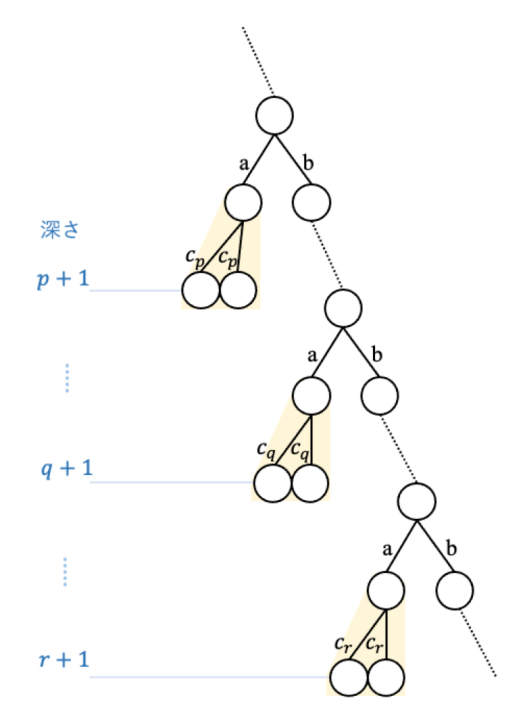
\includegraphics[scale=0.5]{fig/clause-tree.eps}
  \caption{論理変数$x_p,x_q,x_r$ $(1\leq p < q < r \leq n)$のリテラルを含む節$C_k$ $(1\leq k\leq m)$に対する$T$ (図\ref{fig:sample-tree})の変更箇所}\label{fig:clause-tree}
\end{figure}

% 図3.3
\begin{figure*}[tb]
  \centering
  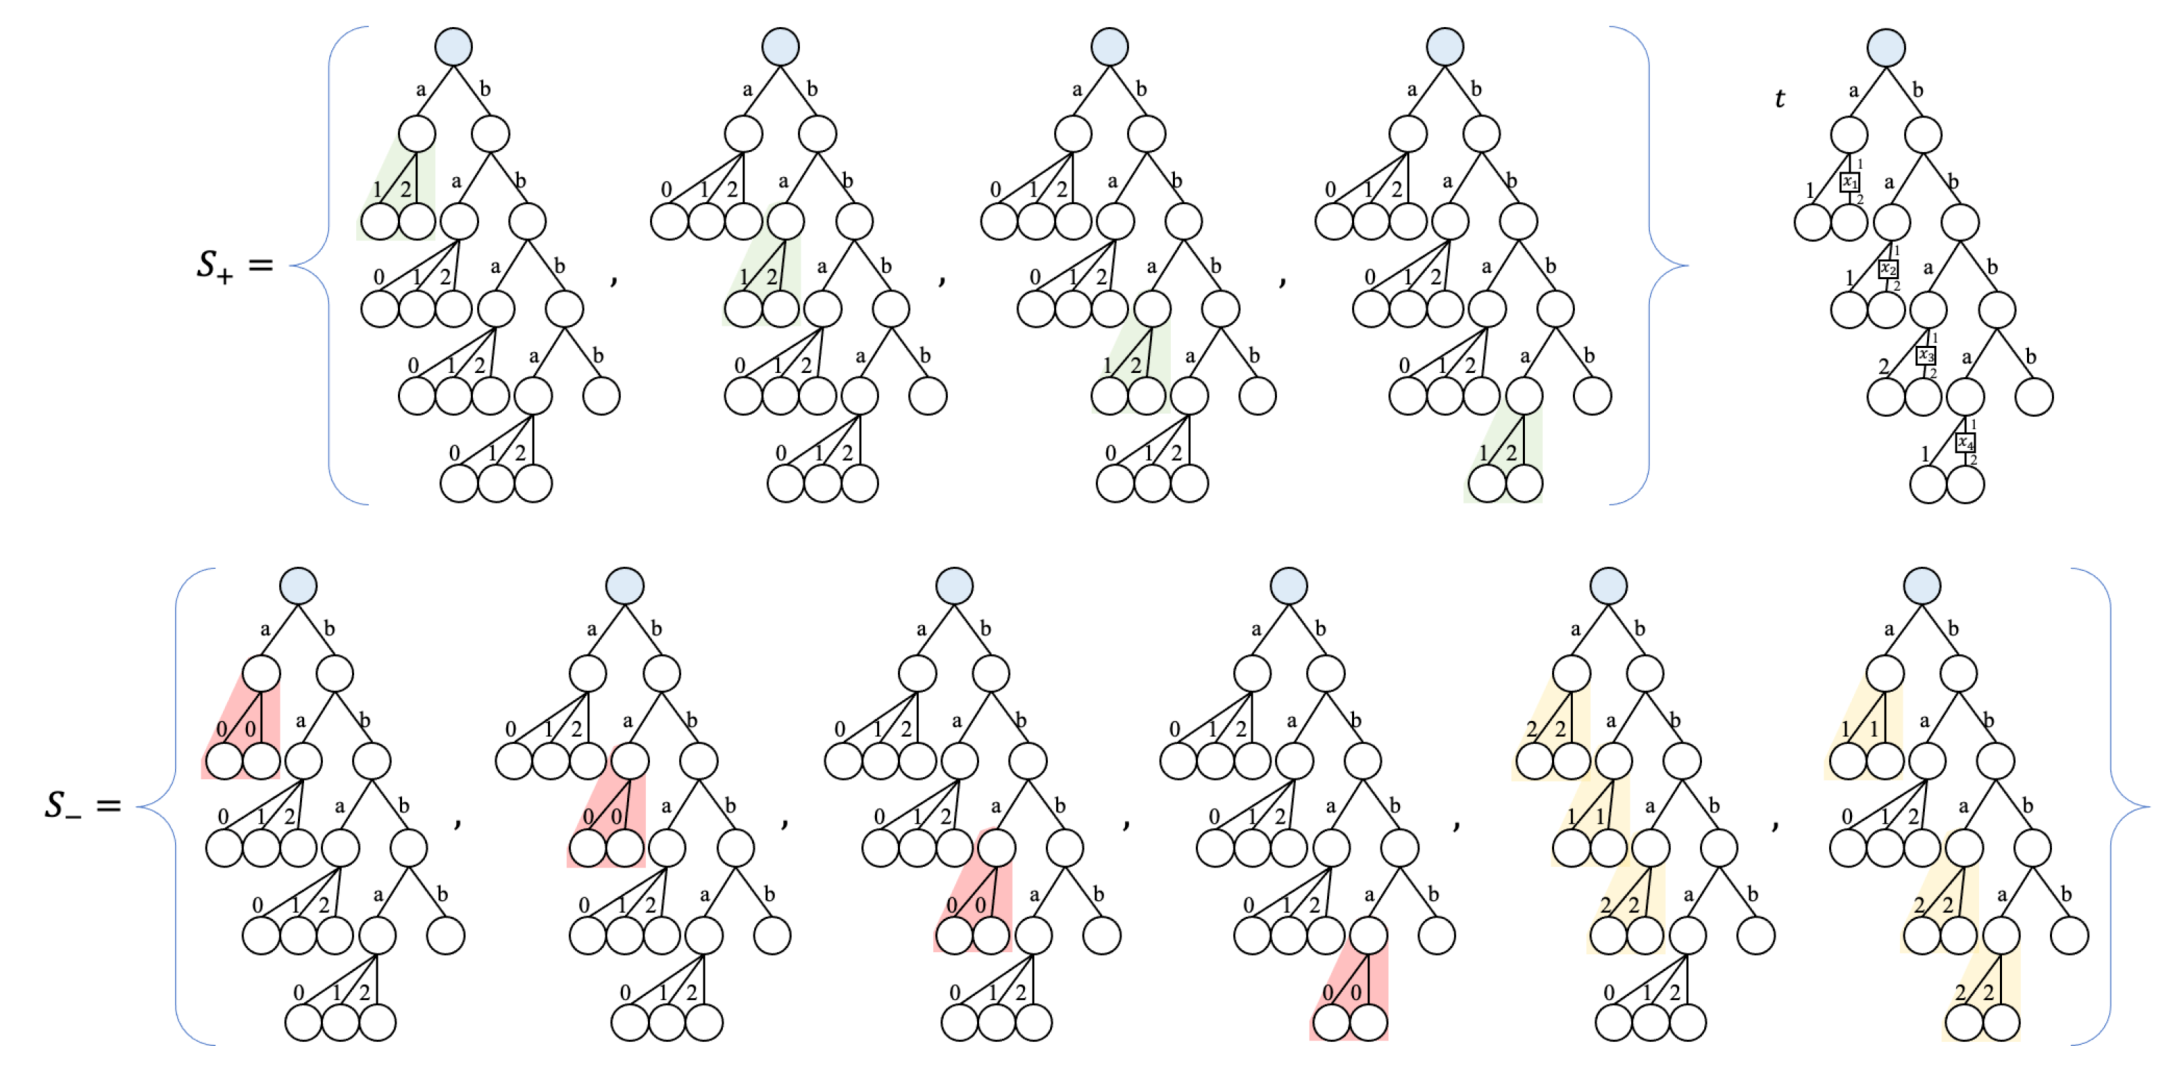
\includegraphics[scale=0.42]{fig/example_npc.eps}
  \caption{多項式時間帰着の例: 3-CNF$F=(x_{1}\vee \bar{x_{2}}\vee x_{3})\wedge(\bar{x_{1}}\vee x_{3}\vee x_{4})$に対する$S_{+}$と$S_{-}$及び,$S_+\subseteq L(t)$かつ$S_-\cap L(t)=\emptyset$を満たす線形無順序木パターン$t\in {\cal LUTP}_{\Sigma,\Lambda,X}$}\label{fig:example_npc}
\end{figure*}

\noindent
\textbf{主張 1.}
3-CNF $F$から$S_{+}, S_{-}$への変換は多項式時間で計算可能である.
\smallskip

\noindent
(主張1の証明)
$F$に現れる論理変数$x_{1},\ldots,x_{n}$から,$T_{1}^{(+)},\ldots,T_{n}^{(+)}$及び$T_{1}^{(-)},\ldots,T_{n}^{(-)}$を得るには,論理変数$x_{i}$に対して,$T$の深さ$i+1$の葉の位置を求めるだけなので,全ての論理変数に対して$n\times O(n) = O(n^{2})$時間で計算することができる.次に,$F$に現れる節$C_k$ $(1\leq k\leq m)$に対して,その節$C_k$が論理変数$x_p,x_q,x_r$ $(1\leq p < q < r \leq n)$のリテラルを含むとき,$T$の深さ$p+1, q+1, r+1$の葉の位置を求めるだけなので,全ての節に対して$m\times O(n) = O(mn)$時間で計算することができる.以上より,この変換は$n$と$m$に関する多項式時間で計算することができる.
(主張1の証明終わり)

\medskip

\noindent
\textbf{主張 2.}
3-CNF $F$を充足可能とする論理変数への論理値割り当てが存在するならば,線形無順序木パターン$t$で$S_{+}\subseteq L(t)$かつ$S_{-}\cap L(t)=\emptyset$となるものが存在する.
\smallskip

\noindent
(主張2の証明)
$F$を充足可能とする論理変数の論理値割り当てにおいて,$x_{i}$ ($1\leq i\leq n$)の論理値が$true$のとき,$T$の深さ$i+1$ ($1\leq i\leq n$)の同じ親を持つ葉の親への辺で辺ラベル$0$の辺を変数とし,$2$を辺ラベルとする親へ辺を持つ葉を削除する.また,$x_{i}$ ($1\leq i\leq n$)の論理値が$false$のとき,$T$の深さ$i+1$ ($1\leq i\leq n$)の同じ親を持つ葉の親への辺で辺ラベル$0$の辺を変数とし,$1$を辺ラベルとする親へ辺を持つ葉を削除する.このようにして,$T$から線形無順序木パターン$t$を構成する.こうして構成した線形無順序木パターンは,$S_{+}$と$S_{-}$の構成方法から,$S_{+}\subseteq L(t)$かつ$S_{-}\cap L(t)=\emptyset$を満たす.
(主張2の証明終わり)

\medskip

\noindent
\textbf{主張 3.}
線形無順序木パターン$t$で$S_{+}\subseteq L(t)$かつ$S_{-}\cap L(t)=\emptyset$となるものが存在すれば,3-CNF $F$を充足可能とする論理変数への論理値割り当てが存在する.
\smallskip

\noindent
(主張3の証明)
線形無順序木パターン$t$が$S_{+}\subseteq L(t)$かつ$S_{-}\cap L(t)=\emptyset$を満たすとする.
$t$の高さ,すなわち葉の深さの最大値は$n+1$でなければならない.なぜなら,$T_{n}^{(+)}\in L(t)$かつ$T_{n}^{(-)}\not\in L(t)$が満たされており,それら2つの無順序木の違いは同じ親を持つ深さ$n+1$の葉の親への辺ラベルだけだからである.
$t$の各頂点の子の数は高々$2$である.
$t$の根は$2$つの子を持つ.
一方の辺ラベルは$a$であり,他方は$b$である.
$a$の辺ラベルを持つ辺で繋がった根からの頂点は高々$2$つの子を持つ.
そのうち1つは,同じ深さで$3$つの子を持つ$T_{2}^{(+)},\ldots,T_{n}^{(+)}$が全て$L(t)$に属することから,変数で繋がった子となる.
一方,もう1つのこは$T_{1}^{(-)}\not\in L(t)$であることから,辺ラベル$1$または$2$を持つ辺で繋がった子である.
同様の議論により,深さ$i+1$ ($2\leq i\leq n$)の同じ親を持つ葉は2つであり,1つは$1$または$2$を辺ラベルとして持つ辺で親と繋がり,他方は変数で親と繋がる.
ここで,深さ$n-1$の葉でない頂点は2つあるが,そのうち1つは辺ラベル$b$を持つ辺で葉と繋がるか,または変数で葉と繋がるかのいずれかである.
この線形無順序木パターン$t$から,次のようにして論理変数$x_{1},\ldots,x_{n}$への論理値割り当てを構成する.
深さ$i+1$ ($1\leq i\leq n$)の同じ親を持つ2つの葉に繋がる変数でない葉の親への辺ラベルが$1$のときは,$x_{i}$の論理値を$true$に,辺ラベルが$2$のときは,$x_{i}$の論理値を$false$にする.この論理値割り当ては,各節$C_{k}$ ($1\leq k\leq m$)に対する無順序木$T_{n+k}^{(-)}$が$L(t)$に含まれないことから,$C_{k}$に現れるリテラルが全て$false$になることはない.
したがって,$S_{+}\subseteq L(t)$かつ$S_{-}\cap L(t)=\emptyset$となる線形無順序木パターン$t$が存在すれば,3-CNF $F$を充足する論理変数の論理値割り当てが存在する.
(主張3の証明終わり)

\medskip

\noindent
主張1,2,3より,${\cal LUTP}$-${\cal CP}$はNP完全である.
\end{proof}

%\end{document}